\begin{tikzpicture}[
    point/.style = {draw, circle, inner sep=2pt},
    truepoint/.style = {point, fill = black},
    trueinterval/.style = {line width = 2pt},
    spanpoint/.style = {point, fill = black, inner sep=1pt},
    spaninterval/.style = {line width = 1pt}
]

\pgfmathsetmacro{\nn}{3}

\pgfmathsetlengthmacro{\labeldist}{8pt}
\pgfmathsetlengthmacro{\spandist}{12pt}

\drawaxis{\nn}{\labeldist}
\drawinterval{001}{110}

\begin{scope}[nodes = {below=\spandist}]
    \drawinterval{001}{001}{$001$};
    \drawinterval{010}{011}{$01 \phi$};
    \drawinterval{100}{101}{$10 \phi$};
    \drawinterval{110}{110}{$110$};
\end{scope}

\end{tikzpicture}